\documentclass[a4paper,12pt]{article} 
\usepackage[T2A]{fontenc}			
\usepackage[utf8]{inputenc}			
\usepackage[english,russian]{babel}
\usepackage{float}
\usepackage{amsmath,amsfonts,amssymb,amsthm,mathrsfs,mathtools} 
\usepackage{cancel}
\usepackage{multirow}
\usepackage[colorlinks, linkcolor = blue]{hyperref}
\usepackage{upgreek}\usepackage[left=2cm,right=2cm,top=2cm,bottom=3cm,bindingoffset=0cm]{geometry}
\usepackage{tikz}
\usepackage{graphicx}
\usepackage{subfig}
\usepackage{titletoc}
\usepackage{pgfplots}
\usepackage{xcolor}
\usepackage{wrapfig}
\usepackage{pgfplots}
\pgfplotsset{width=10cm,compat=1.9}

\begin{document}

\begin{titlepage}
		\vspace*{\fill}
		
		\begin{center}
			
\includegraphics[scale=0.8]{MIPT.pdf}
			\\[0.7cm]\Huge Московский Физико-Технический Институт
			\\[2cm]\LARGE Отчет по эксперименту
			\\[0.5cm]\noindent\rule{\textwidth}{1pt}
			\\\Huge\textbf{4.3.4. \\ Преобразование Фурье в оптике}
			\\[-0.5cm]\noindent\rule{\textwidth}{1pt}
		\end{center}
		
		\vspace*{\fill}
		
		\begin{flushleft}
			Выполнила: \hspace{\fill} Группа:
			\\Малиновская София \hspace{\fill} Б05-102
		\end{flushleft}
	\end{titlepage}

	\setcounter{page}{2}

\section*{Цель работы} 
Исследовать преобразование Фурье в оптике: определить периоды решеток и ширину щели по их спектру и явление мультиплицирования.


\section*{В работе используются} 
Гелий-неоновый лазер с длиной волны $\lambda = 6328 \cdot 10^{-10}$ м, кассета с набором
сеток разного периода, щель с микрометрическим винтом, линзы,
экран, линейка.


\section*{Теоретическая сводка}
Сложное волновое поле во многих случаях удобно анализировать, разлагая его на простейшие составляющие, в частности представляя его в виде разложения по плоским волнам. При этом оказывается, что если мы рассматриваем поле, полученное после прохождения плоской монохроматической волны через предмет с функцией пропускания $\tau(x)$, то разложение по плоским волнам соответствует преобразованию Фурье от этой функции. Если за предметом поставить линзу, то каждая плоская волна сфокусируется в свою точку в задней фокальной плоскости линзы. Таким образом, картина, наблюдаемая в фокальной плоскости линзы, даёт нам представление о спектре плоских волн падающего на линзу волнового поля. Поэтому можно утверждать, что с помощью линзы в оптике осуществляется пространственное преобразование Фурье.

\noindent
Если мы установим в задней фокальной плоскости линзы решетку, то будем наблюдать явление мультипликаиции. При этом вместо изображения одиночного предмета мы будем наблюдать экивдистантный набор изображений таких предметов. Для этого необходимо, чтобы период решетки был заметно меньше ширины спектра. Поменяв местами сетку и щель, можно исследовать влияние размера щели на изображение сетки.


\section*{Ход работы}
\paragraph{Определение ширины щели} cначала определим ширину щели следующим способом: на экране Э получим изображение щели D, освещаемой параллельным пучком света, излучаемого лазером, с помощью линзы Л$_1$. Схема этой установки изображена на рис. 1. Будем измерять размер изображения щели $D_1$ в зависимости от ширины щели $D$. Результаты занесены в таблицу 1, по ним построим график, изображенный на рис. 2.

\begin{figure}[H]
    \centering
    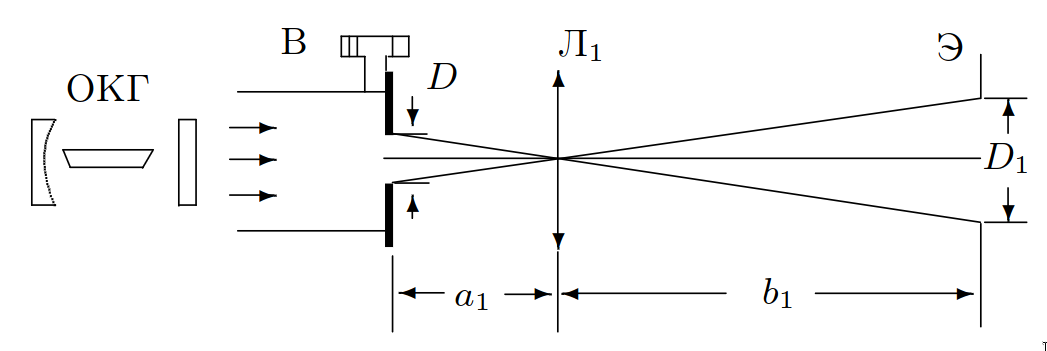
\includegraphics[scale=0.3]{image_1_.png}
    \caption{Схема установки для определения ширины щели по увеличенному изображению}
\end{figure}

\noindent
Прежде всего, определим начало отсчета по открытию щели: $D_0 = 0.70$ мм. Будем считать это положение щели нулем и отсчитывать ширину от него. Погрешность измерения $D_1$ составляет 1 мм, $D$ --- 0.01 мм.

\begin{table}[H]
    \centering
    \caption{Зависимость размера изображения щели от ее ширины}
    \begin{tabular}{|c|c|} \hline
        $D,$ мм & $D_1,$ мм \\ \hline
        0 & 0 \\ \hline
        0.05 & 2 \\ \hline
        0.10 & 3 \\ \hline
        0.15 & 4 \\ \hline
        0.20 & 5 \\ \hline
        0.25 & 6 \\ \hline
        0.30 & 7 \\ \hline
        0.35 & 8 \\ \hline
        0.40 & 9 \\ \hline
        0.45 & 10 \\ \hline
        0.50 & 12 \\ \hline
        0.60 & 15 \\ \hline
        0.70 & 17 \\ \hline
    \end{tabular}
\end{table}

\begin{figure}[H]
    \centering
    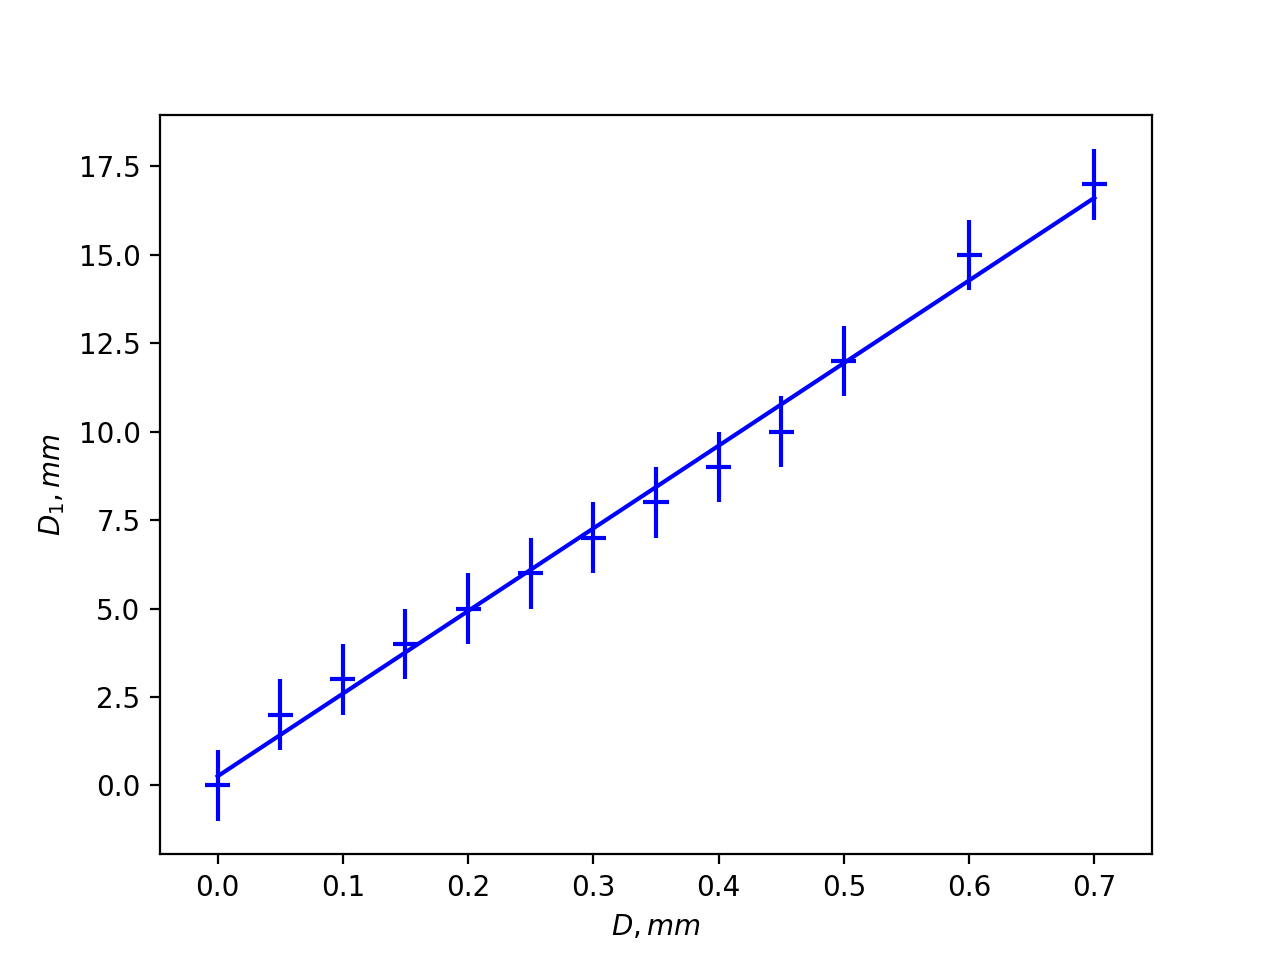
\includegraphics[scale=0.5]{I.png}
    \caption{Зависимость размера изображения от ширины щели}
\end{figure}

\noindent
Из графика найдем $\Gamma = 23.4 \pm 2.0$.

\noindent
Размер изображения щели также можно найти по следующей формуле
\[
    \Gamma = \frac{D_1}{D} = \frac{b_1}{a_1},
\]
где $D$ --- ширина щели, $D_1$ --- размер изображения щели, $a_1$ --- расстояние от щели до линзы, $b_1$ --- расстояние от линзы до экрана.

\noindent
Измерив значения $a_1  = 4.5 \pm 0.5$ см, $b_1 = 127.0 \pm 2.0$ см, вычислим величину $\Gamma = 28.0 \pm 4.5$. Этот метод является менее точным из-за большой погрешности измерения расстояния, но в пределах погрешности измеренные величины совпадают.

\begin{figure}[H]
    \centering
    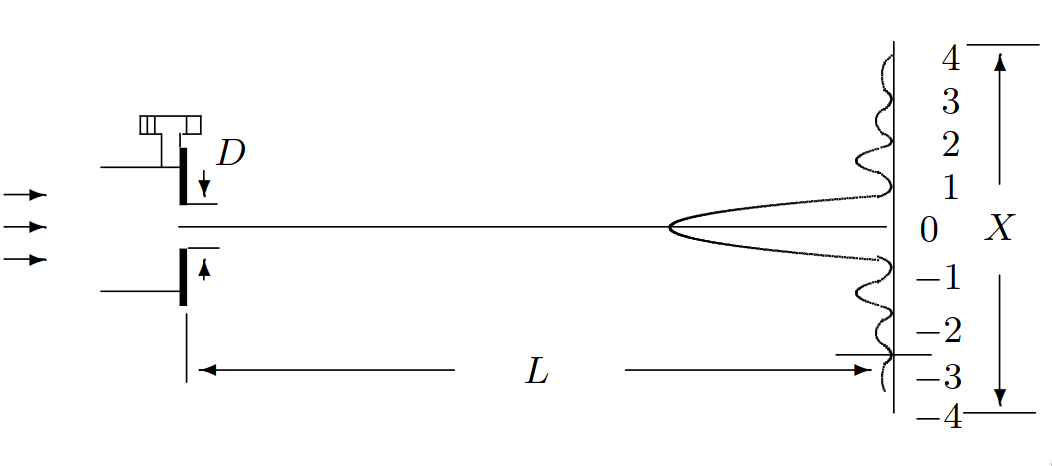
\includegraphics[scale=0.3]{image_2_.png}
    \caption{Схема установки для определения ширины щели по ее спектру}
\end{figure}

\noindent
Теперь определим ширину щели вторым способом: по ее спектру. Для этого соберем установку согласно схеме, представленной на рис. 3, которая отличается от предыдущей лишь отсутствием линзы. Будем проводить измерения ширины спектра в зависимости от ширины щели. Для этого измерим расстояние $X$ между минимумами, удаленными от центра, и порядковый номер соответствующего минимума $m$. По фомуле (1) рассчитаем величину $D_\text{с}$ --- ширину щели. Результаты измерений представлены в таблице 2. Расстояние от лазера до экрана составляет $L = 132 \pm 1$ см.

\begin{equation}
    \Delta X = \frac{X}{2m} = \frac{\lambda}{D_\text{с}} L
\end{equation}

\begin{table}[H]
    \centering
    \caption{Зависимость ширины спектра от ширины линзы}
    \begin{tabular}{|c|c|c|c|} \hline
        $D,$ мм & $m$ & $X,$ мм & $D_\text{с}$ \\ \hline
        0.05 & 3 & 78 &  0.06 \\ \hline 
        0.10 & 6 & 65 &  0.11 \\ \hline 
        0.15 & 9 & 75 &  0.15 \\ \hline 
        0.20 & 12 & 72 & 0.20 \\ \hline 
        0.25 & 13 & 71 & 0.27 \\ \hline 
        0.30 & 14 & 62 & 0.30 \\ \hline 
        0.35 & 17 & 60 & 0.37 \\ \hline 
    \end{tabular}
\end{table}

\noindent
Построим на одном графике зависимсоти $D_\text{л}$ от $D$ и $D_\text{с} = \frac{a_1}{b_1}D_1$ от $D$. Этот график представлен на рис. 4.

\begin{figure}[H]
    \centering
    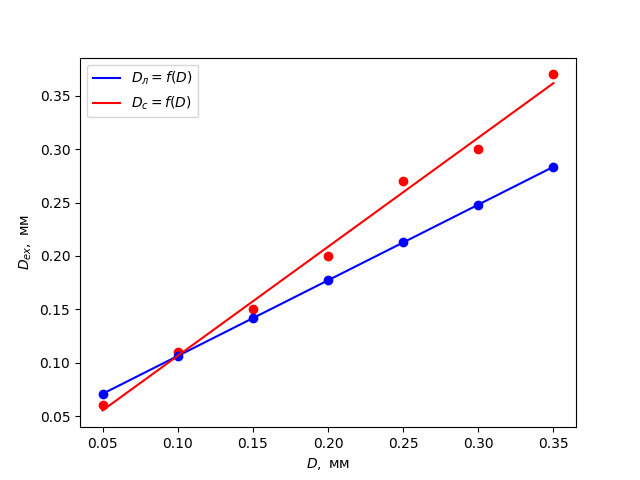
\includegraphics[scale=0.5]{II.png}
    \caption{Зависимость измеренной ширины щели от фактической}
\end{figure}

\noindent 
Первый способ является менее точным, поскольку $\Gamma$ измерена лишь с большой погрешностью. Этим объясняется то, что зависимости на рис. 4 имеют разный наклон.

\paragraph{Определение периода решеток} поставим кассету с решетками вплотную к выходному окну лазера и измерим для каждой сетки расстояние $X$ между $m$-тыми максимумами и сам номер максимума $m$. Также рассчитаем период решетки по формуле (2). Результаты занесены в таблицу 3.

\begin{equation}
    \Delta X = \frac{X}{2m} = \frac{\lambda}{d_c}L
\end{equation}

\begin{table}[H]
    \centering
    \caption{Измерение периода решеток по спекру на удаленном экране}
    \begin{tabular}{|c|c|c|c|} \hline
        номер сетки & $X,$ мм & $m$ & $d_c,$ мкм \\ \hline
        1, низ & 145 & 2 & $11.5 \pm 0.1$ \\ \hline
        1, верх & 145 & 2 & $11.5 \pm 0.1$ \\ \hline
        2, низ & 147 & 5 & $28.4 \pm 0.2$ \\ \hline
        2, верз & 147 & 5 & $28.4 \pm 0.2$ \\ \hline
        3, низ & 72 & 5 & $58.0 \pm 0.1$ \\ \hline
        3, верх & 72 & 5 & $58.0 \pm 0.1$ \\ \hline
    \end{tabular}
\end{table}

\noindent
Можно утверждать, что верхние и нижние сетки для каждого номера одинаковы, так как дают одинаковый спектр. Далее будут проводится измерения лишь для верхних сеток. 

\noindent
Теперь проведем измерения периода решеток другим способом. Для этого соберем схему, представленную на рис. 5. Здесь линза Л$_2$ совершает прямое преобразование Фурье, а линза Л$_3$ дает на экране увеличенное изображение спектра. Проведем измерения, аналогичные предыдущим, а также рассчитаем период решетки по форумле (3) и занесем занесем в таблицу 4.

\begin{figure}[H]
    \centering
    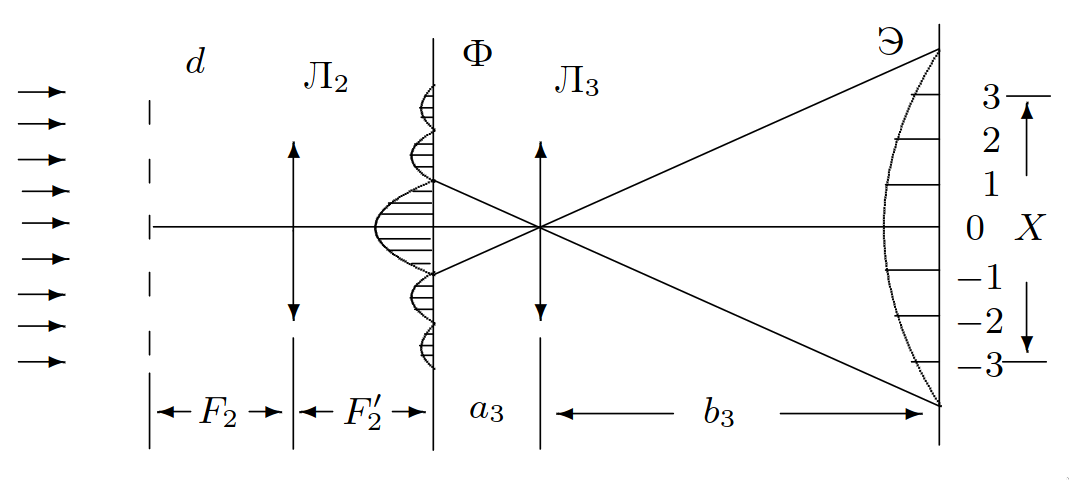
\includegraphics[scale=0.30]{image_3_.png}
    \caption{Схема установки для определения периода решетки по увеличенному изображению спектра}
\end{figure}

\begin{equation}
    \Delta X = \frac{X}{\Gamma_3} = \frac{\lambda}{d_\text{л}} F_2
\end{equation}
\noindent
Здесь $F_2 = 11$ см --- фокусное расстояние линзы, $\Gamma_3 = 3.5 \pm 0.5$ --- увеличение линзы Л$_3$, $\Delta X$ --- расстояние между максимума.

\begin{table}[H]
    \centering
    \caption{Измерение периода решеток по увеличенному изображению спектра}
    \begin{tabular}{|c|c|c|c|} \hline
        номер сетки & $X,$ мм & $m$ & $d_\text{л},$ мкм \\ \hline
        1 & 341 & 1 & $11.1 \pm 2.2$ \\ \hline
        2 & 257 & 2 & $29.5 \pm 3.1$ \\ \hline
        3 & 180 & 3 & $63.3 \pm 4.4$ \\ \hline
    \end{tabular}
\end{table}

\paragraph{Мультиплицирование} соберем схему согласно рис. 6. Для этого снова поставим щель вплотную к окну лазера и найдем на экране резкое изображение щели с помощью линзы Л$_2$. Затем расположим в фокальной плоскости линзы кассету с решетками. Подберем ширину щели так, чтобы на экране можно было наблюдать мультиплицированное изображение для всех сеток. Снимем зависимость расстояния между удаленными изображениями щели $Y$ и числа промежутков между изображениями $K$ от номера сетки. Рассчитаем величину $\Delta y = \Delta Y / \Gamma_2$, где $\Gamma_2 = 10.4$ и $\Delta Y = Y / K$. Результаты представлены в таблице 5.

\begin{figure}[H]
    \centering
    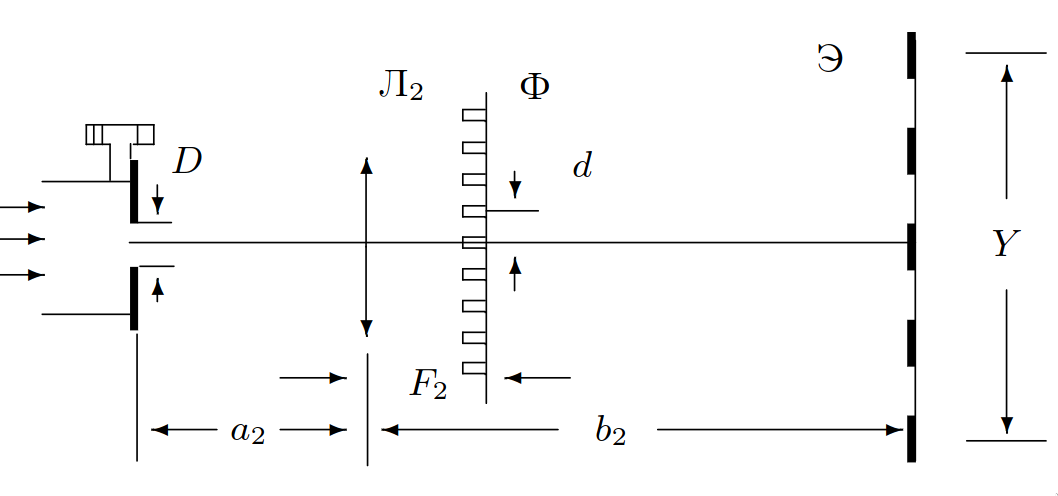
\includegraphics[scale=0.3]{image_4_.png}
    \caption{Схема установки для изучения мультиплицирования}
\end{figure}

\begin{table}[H]
    \centering
    \caption{Зависимость расстояния между удаленными изображениями от числе промежутков при мультиплицировании}
    \begin{tabular}{|c|c|c|c|c|} \hline
        номер сетки & $Y,$ мм & $K$ & $\Delta Y,$ мм & $\Delta y,$ мм \\ \hline
        1 & 119 & 2 & 59.5 & 5.7 \\ \hline
        2 & 118 & 5 & 23.6 & 2.3 \\ \hline
        3 & 70 & 6 & 11.7 & 1.3 \\ \hline
    \end{tabular}
\end{table}

\noindent Построим график зависимости $\Delta y$ от $1/d_\text{с}$. Он изображен на рис. 7. Эта зависимость должны быть линейной, поскольку 
\begin{equation}
    \frac{\lambda}{\Delta y} F_2 = d_c
\end{equation}
Это соотношение вытекает их того, что <<фиктивная>> решетка, изобраение которой мы будто бы видим на экране, расположена в фокусе линзы, значит 
\[
    \frac{\Delta y}{F_2} = \frac{\Omega}{k} = \frac{2\pi / d_c}{2\pi / \lambda} = \frac{\lambda}{d_c}
\]

\noindent
Из графика получаем коэффициент наклона $k = 0.0637$ мм$^2$, в то время как теоретическое значение составляет $\lambda F_2 = 0.0696$ мм$^2$. При этом зависимость дейстивтельно линейна.

\begin{figure}[H]
    \centering
    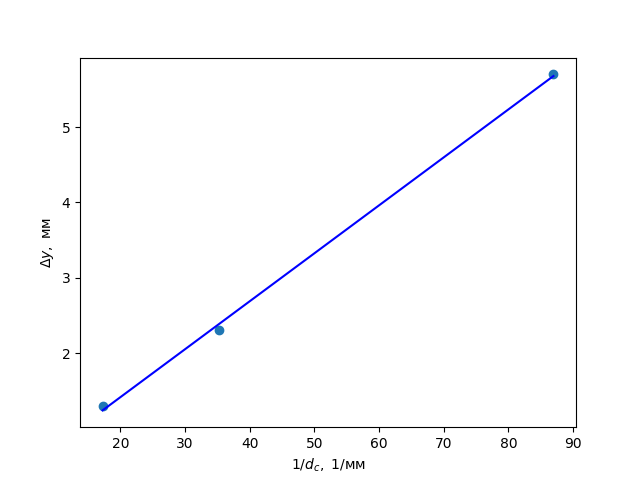
\includegraphics[scale=0.5]{III.png}
    \caption{Зависимость $\Delta y$ от $1/d_\text{с}$}
\end{figure}

\paragraph{Влияние щелевой диафрагмы на изображение сетки} поставим сетку вплотную к окну лазера и с помощью линзы получим четкое изображение сетки на экране. Затем поставим в фокальную плоскость линзы щель и пронаблюдаем, что получится при горизонтальной, вертикальной ориентции щели, а также при расположении щели под углом $45^\circ$ к горизонту. Полученные изображения представлены на рис. 8 Картины для горизонтальной и вертикальной отличаются только ориентацией полос, в то время как картина для щели повернутой под $45^\circ$ к горизонту отличается еще и периодом. Это связано с тем, что при повороте на $45^\circ$ расстояние между максимумами, пропускаемыми щелью возрастает, а значит период дифракционной картины должен убывать, так как можно считать, что линза совершает преобразование Фурье, образ которого имеет тем меньший период, чем больше период прообраза.

\begin{figure}[H]
    \centering
    \begin{minipage}[b]{0.3\textwidth}
        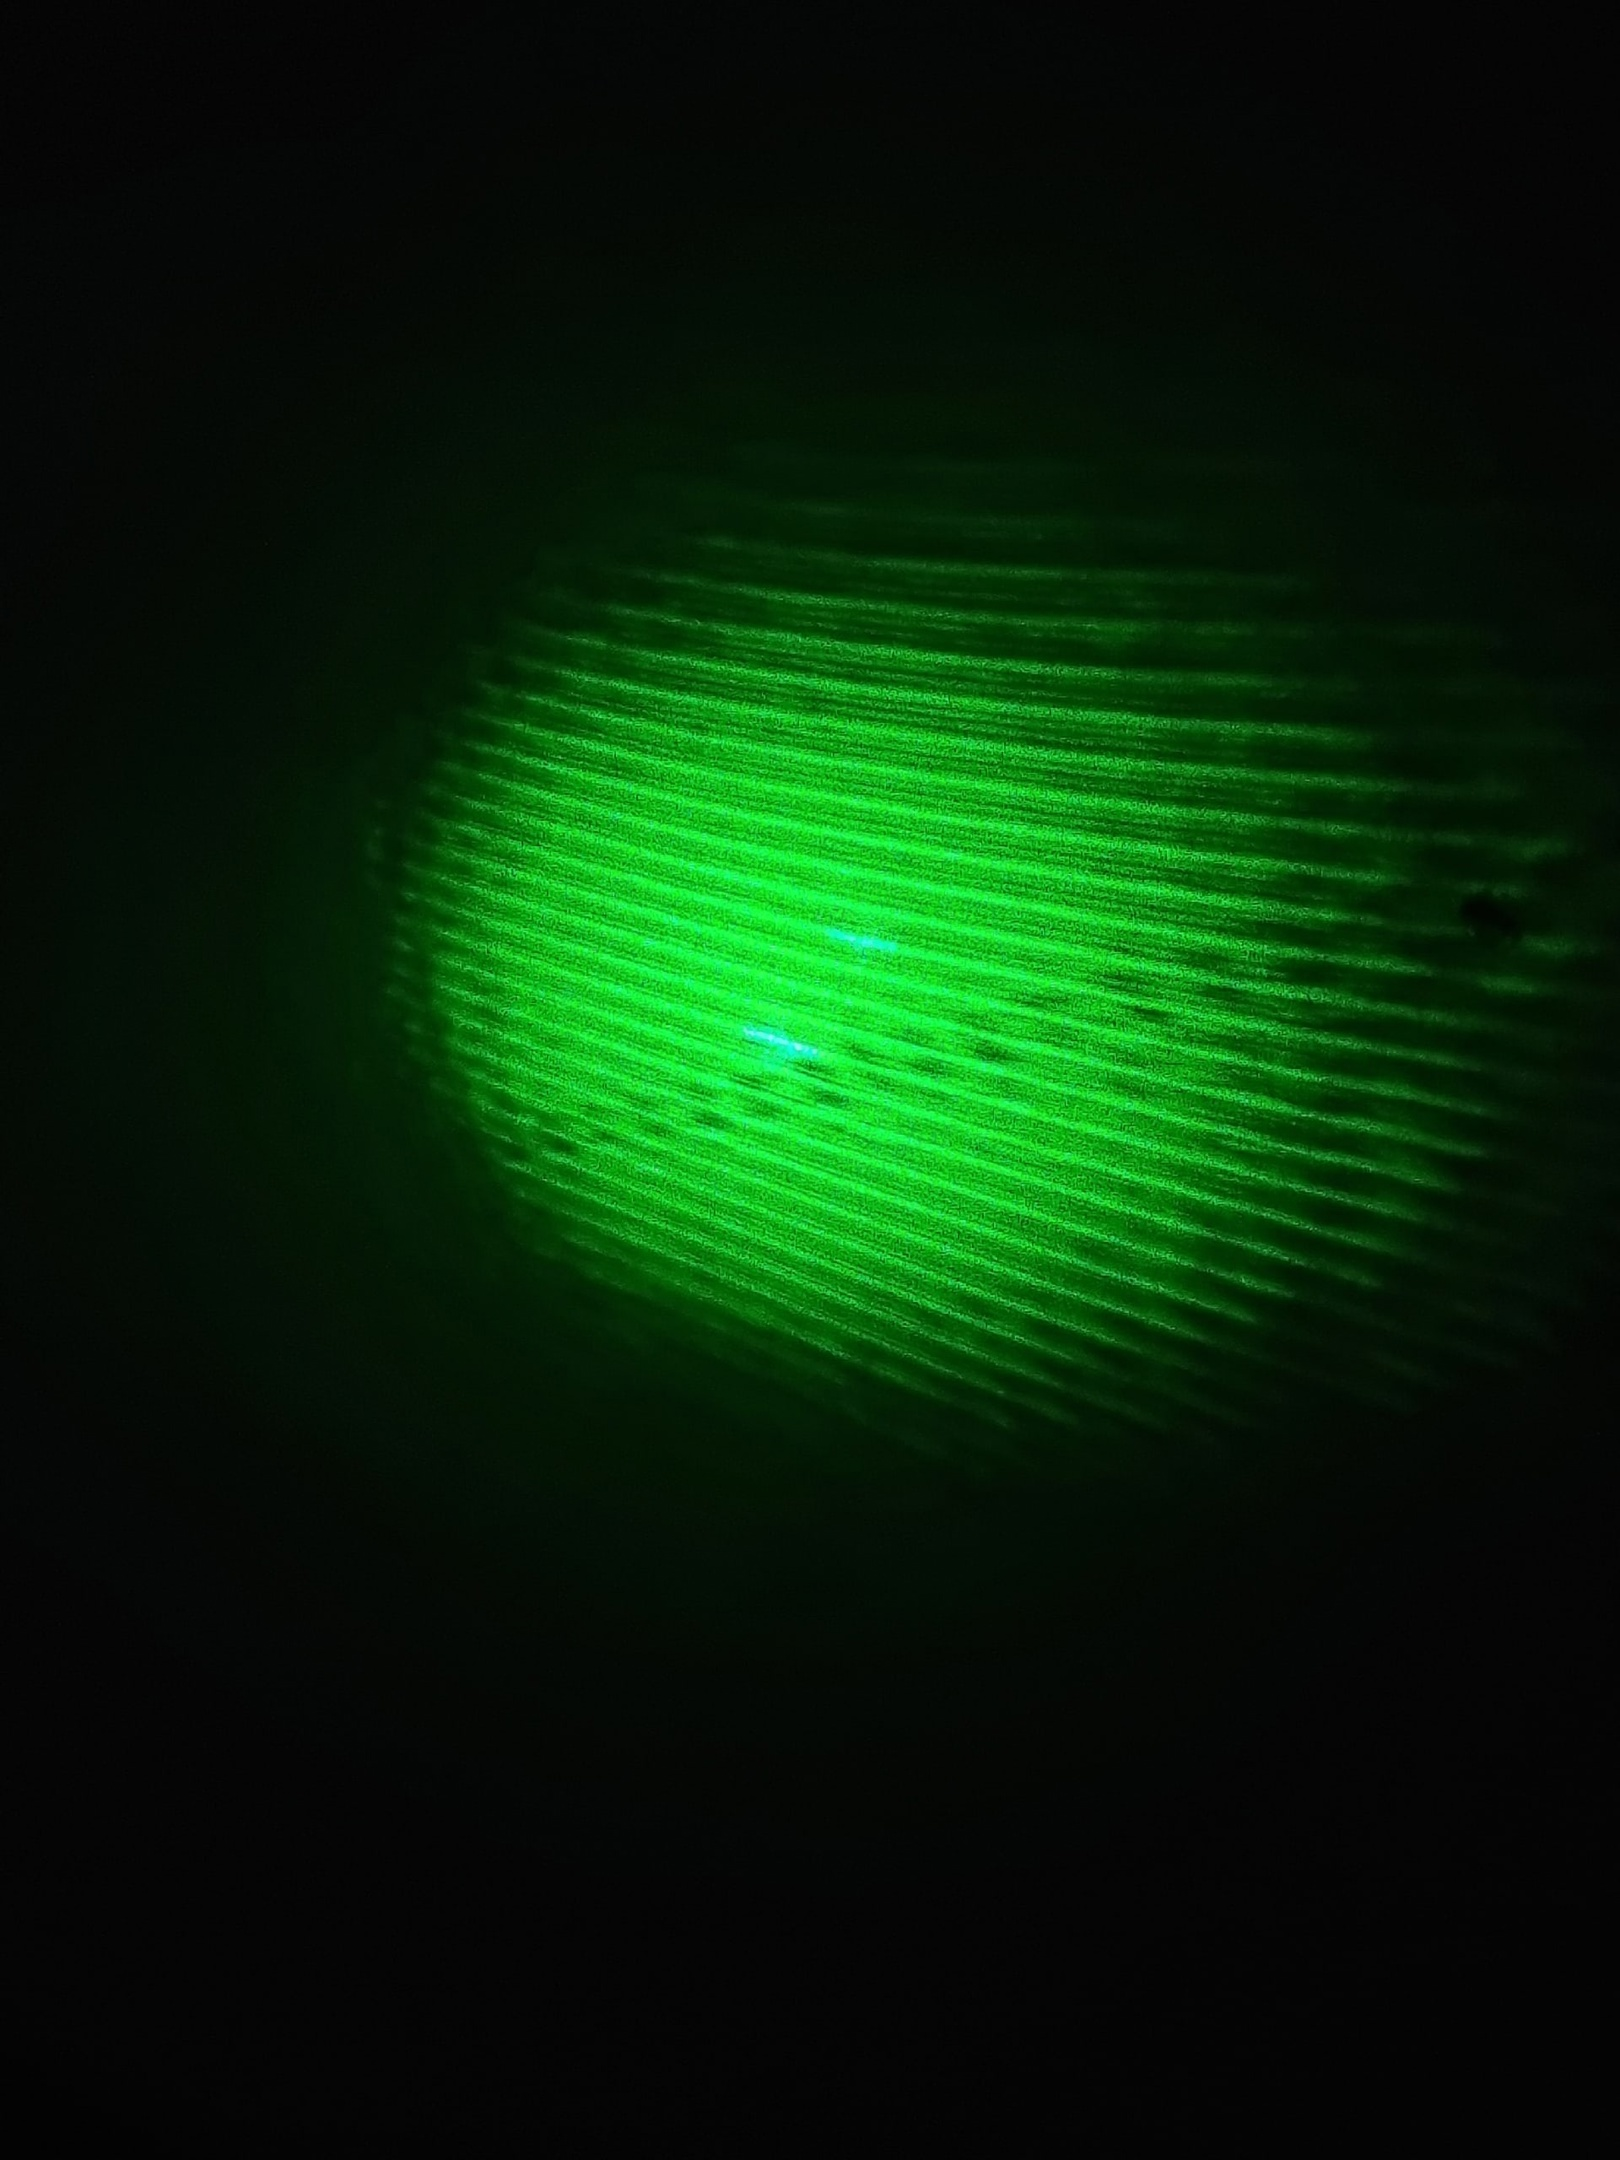
\includegraphics[scale=0.08]{pic_1.png}
        \caption*{(a)}
    \end{minipage}
    \begin{minipage}[b]{0.3\textwidth}
        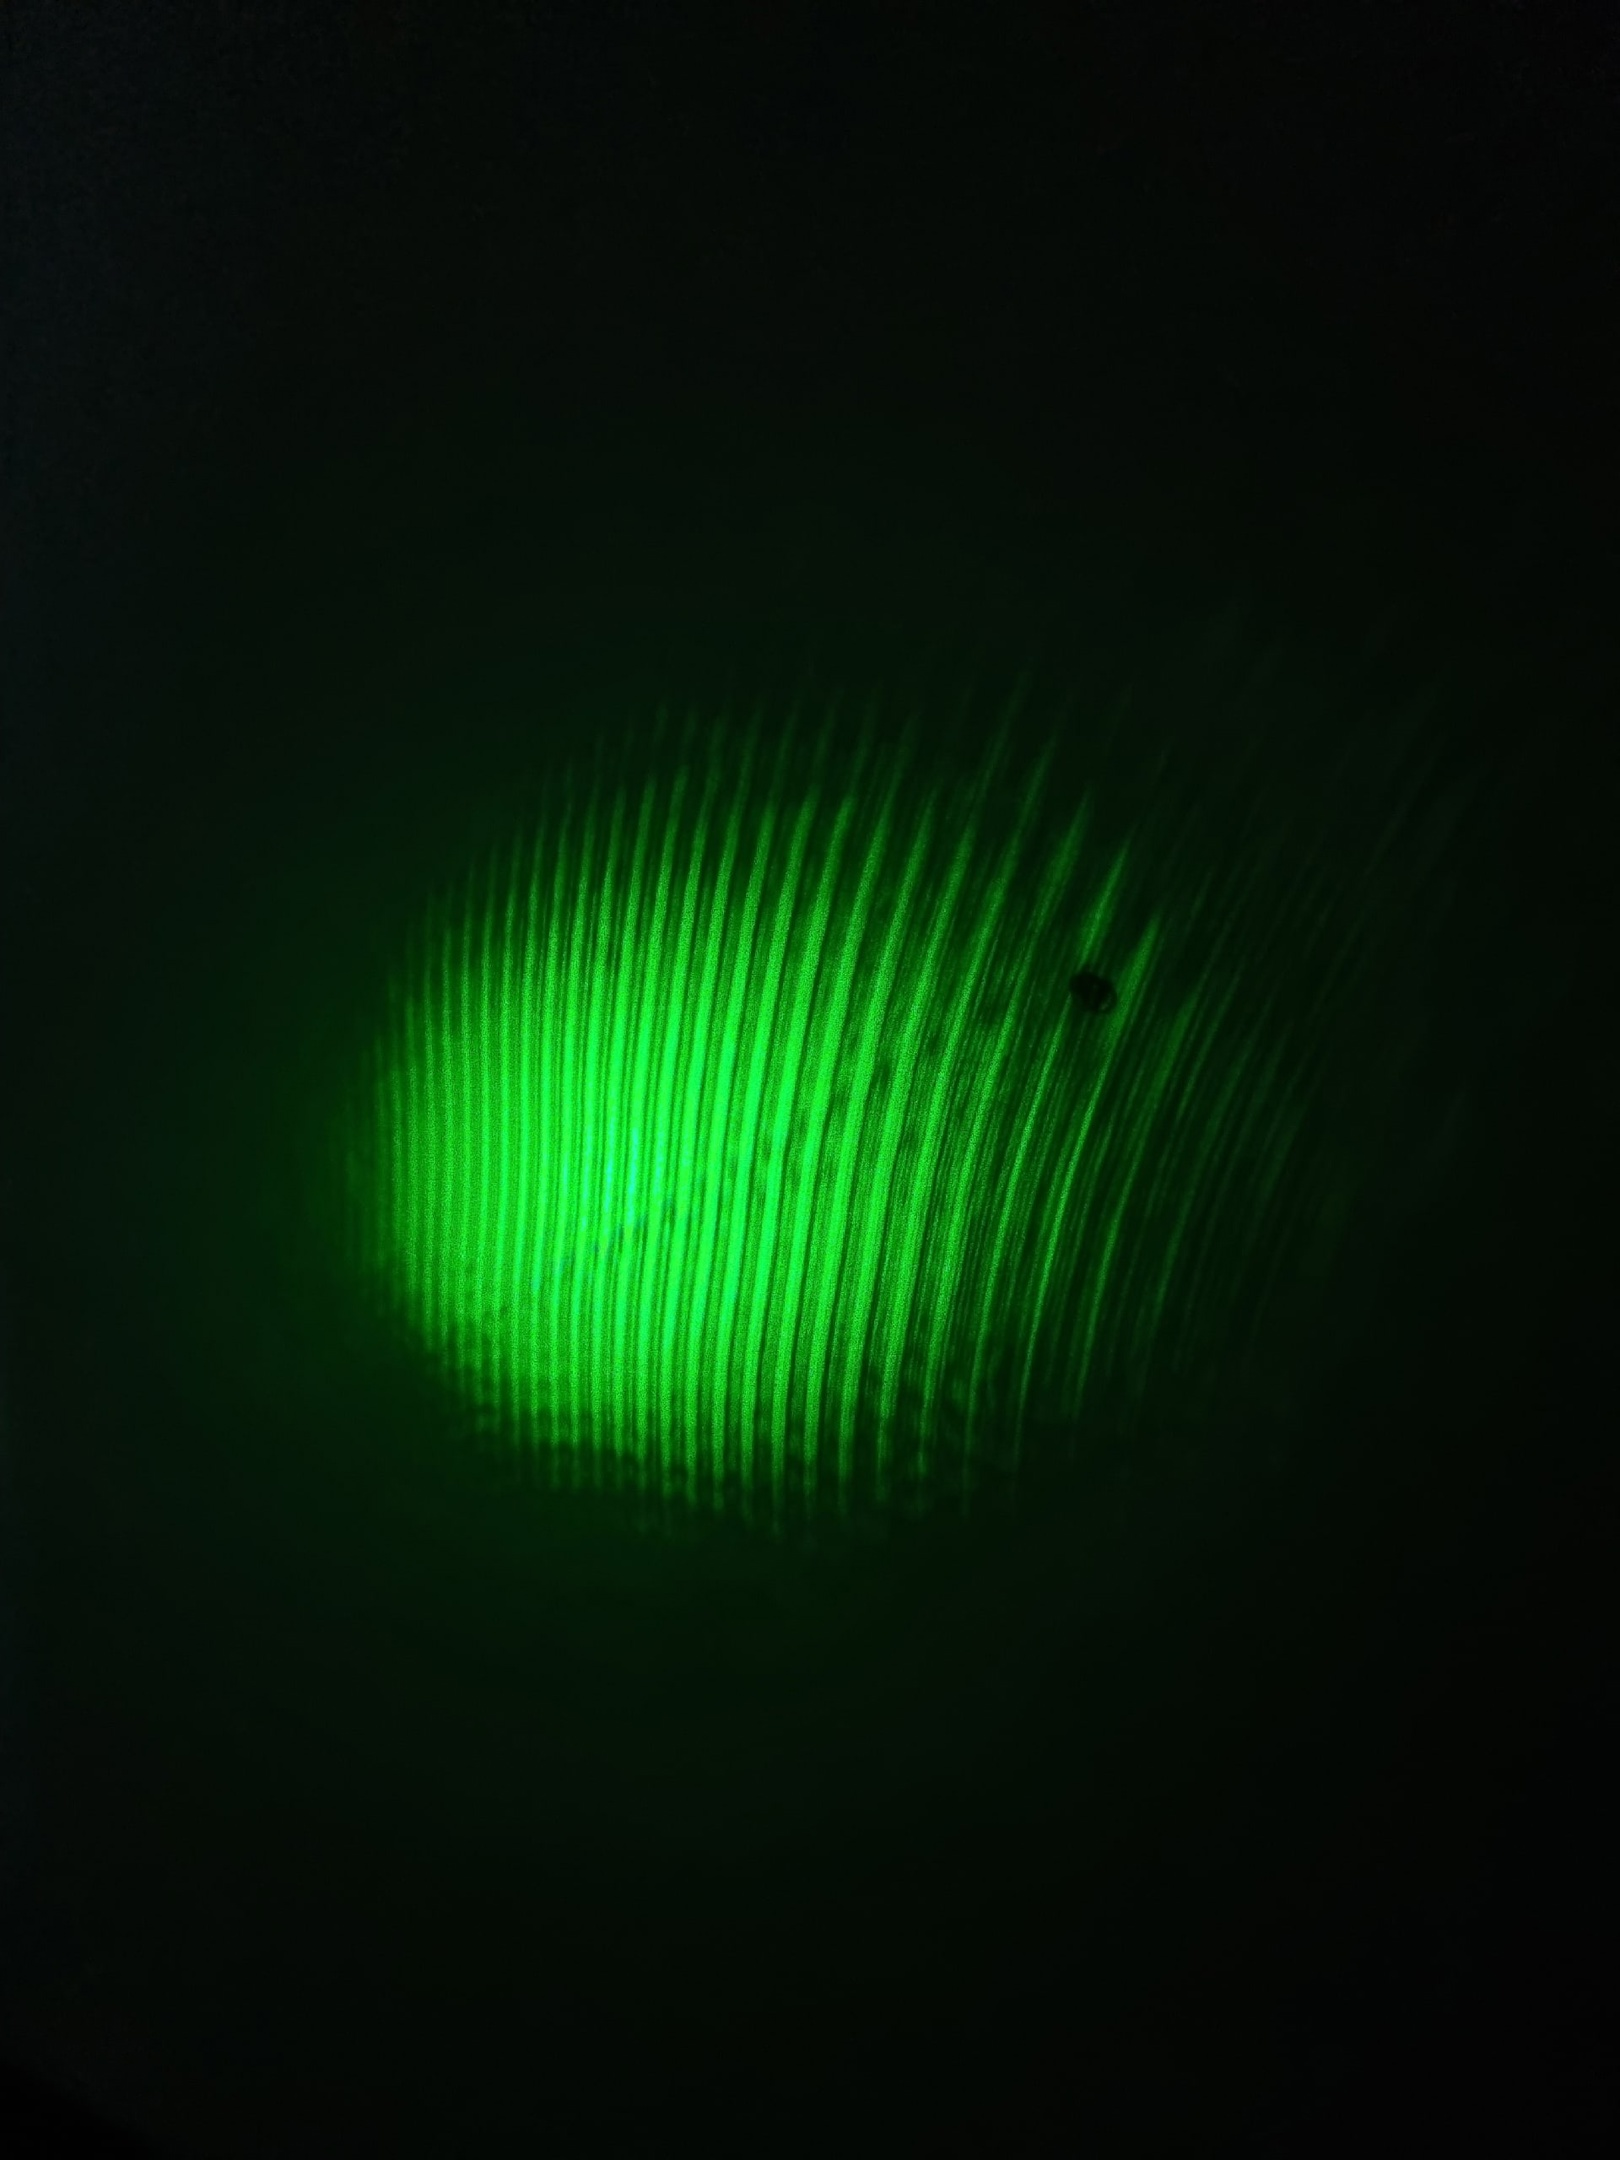
\includegraphics[scale=0.08]{pic_2.png}
        \caption*{(b)}
    \end{minipage}
    \begin{minipage}[b]{0.3\textwidth}
        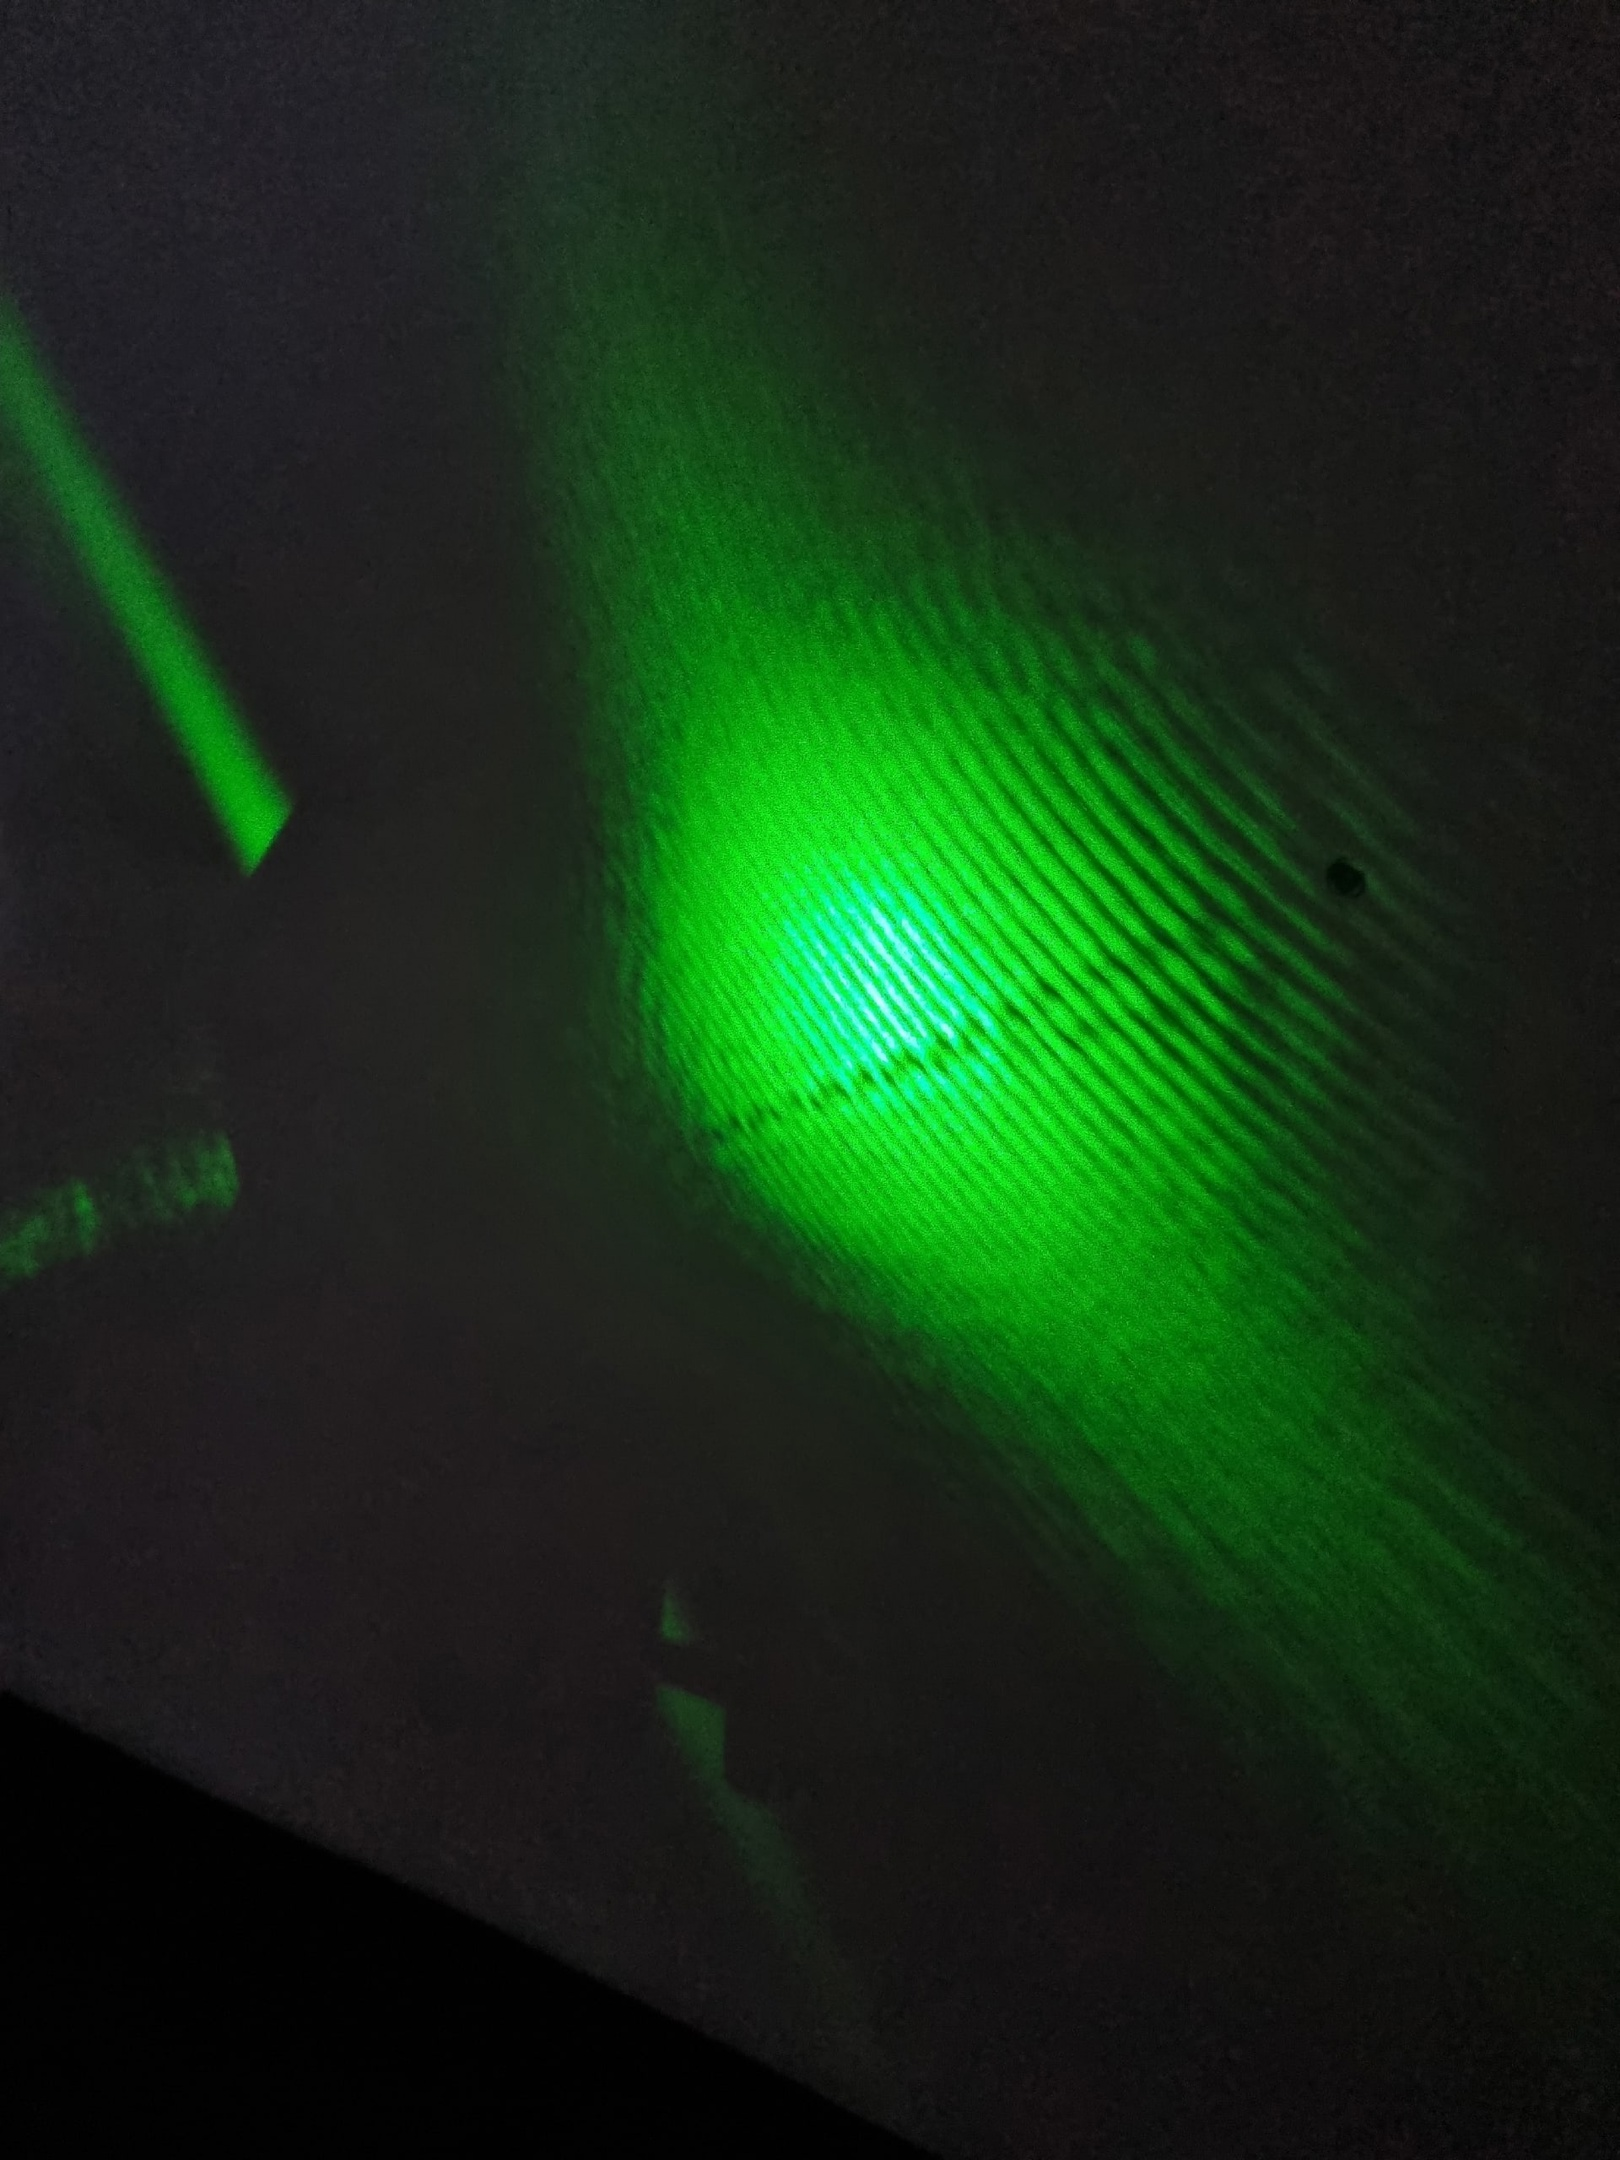
\includegraphics[scale=0.08]{pic_3.png}
        \caption*{(c)}
    \end{minipage}
    \caption{
        (a) --- вертикально ориентированная щель
        (b) --- горизонтально ориентированная щель
        (c) --- щель, ориетированная под $45^\circ$ к горизонту
    }
\end{figure}


\section*{Вывод}
В работе измерялась ширина щели несколькими способами: по увеличенному изображению и по ее спектру. Результаты этих измерений представлены на рис. 4. Зависимость, полученная каждым из способов является линейной, но различаются коэффициенты наклона соответствующих прямых, равные соответственно $1.02$ и $0.71$ для измерений по спектру и увеличенному изображению. Теоретически, коэффициент наклона данной прямой должен быть равен 1, поскольку это зависимость ширины измеренной ширины щели от реальной ширины щели. Наибольшую погрешность в результат вносят неточности измерения длин и увеличения линзы.

\noindent
Также несколькими способами были измерены периоды решеток
\begin{itemize}
    \item при измерении периода решеток по спектру на удаленном экране получены значения $d_1 = 11.5 \pm 0.1$ мкм, $d_2 = 28.4 \pm 0.2$ мкм, $d_3 = 58.0 \pm 0.1$ мкм.
    \item при измерении периода решеток по увеличенному изображению спектра получены значения $d_1 = 11.1 \pm 2.2$ мкм, $d_2 = 29.5 \pm 3.1$ мкм, $d_3 = 63.3 \pm 4.4$ мкм.
\end{itemize}
Различие в полученных значениях в основном объясняется неточностью измерения расстояний, и как следвствие неточностью измерения увеличения линзы.

\noindent
Было проделано мультиплицирование изображения линзы и проверена зависимость (4). Эксперимнтально полученная зависимость, представленная на рис. 7, является линейной с коэффициентом $k = 0.0637$ мм$^2$, в то время как теоретическое значение составляет $\lambda F_2 = 0.0696$ мм$^2$. Можем считать, что теоретическая зависимость подтверждена, поскольку зависимость на рис. 7 построена всего по 3 точкам, а потому может быть достаточно неточной. Также на результат влияет неточность измерения длин, а значит и $\Delta y$, как и во всех прочих частях эксперимента.

\end{document}
